\begin{compactenum}[a)]
\item \emph{Scientific objectives} 
The epidermal growth factor receptor (EGFR) is an especially important enzyme target in lung cancer therapy because it mutates and/or is overexpressed in most non-small cell lung carcinoma (NSCLC) tumours. Inhibition of kinase activation of EGFR is a frequently used method to suppress its functions \cite{bib:nature_tki}. The majority of tyrosine kinase inhibitors (TKIs) are ATP-competitive inhibitors which bind in the ATP-binding site. Molecular dynamics (MD) simulations will be used to study the structural and energetic properties of inhibitor-EGFR complexes. The binding affinity of inhibitors to EGFRs will be calculated by molecular mechanics Poisson-Boltzmann surface area (MM/PBSA) methods \cite{bib:wan_philtrans}. This molecular level study is one component of the EU FP7 ContraCancrum (Clinically Oriented Translational Cancer Multilevel Modeling) project which aims at developing a composite multilevel platform for simulating malignant tumor development and pharmacologic responses to a therapeutic intervention (http://www.contracancrum.eu). We have employed large scale MD techniques using both TeraGrid and DEISA resources in order to study the interactions of inhibitors with wild-type and mutant EGFRs \cite{bib:wc2009}. A better understanding of the reasons for the success or failure of a therapeutic intervention will help us in the selection of subgroups of patients who are most likely to respond to specific drugs, and paves the way for personalized treatment \cite{bib:hiv}. We have already performed a preliminary study of different inhibitors (AEE788, AFN941 and gefitinib) with EGFR which we now intend to extend to look at a wider variety of inhibitors and EGFR mutations and to probe longer time scale motions of the protein.

%\item \emph{Benchmark Data}
%\begin{comment}
%\begin{figure}
%\centering
%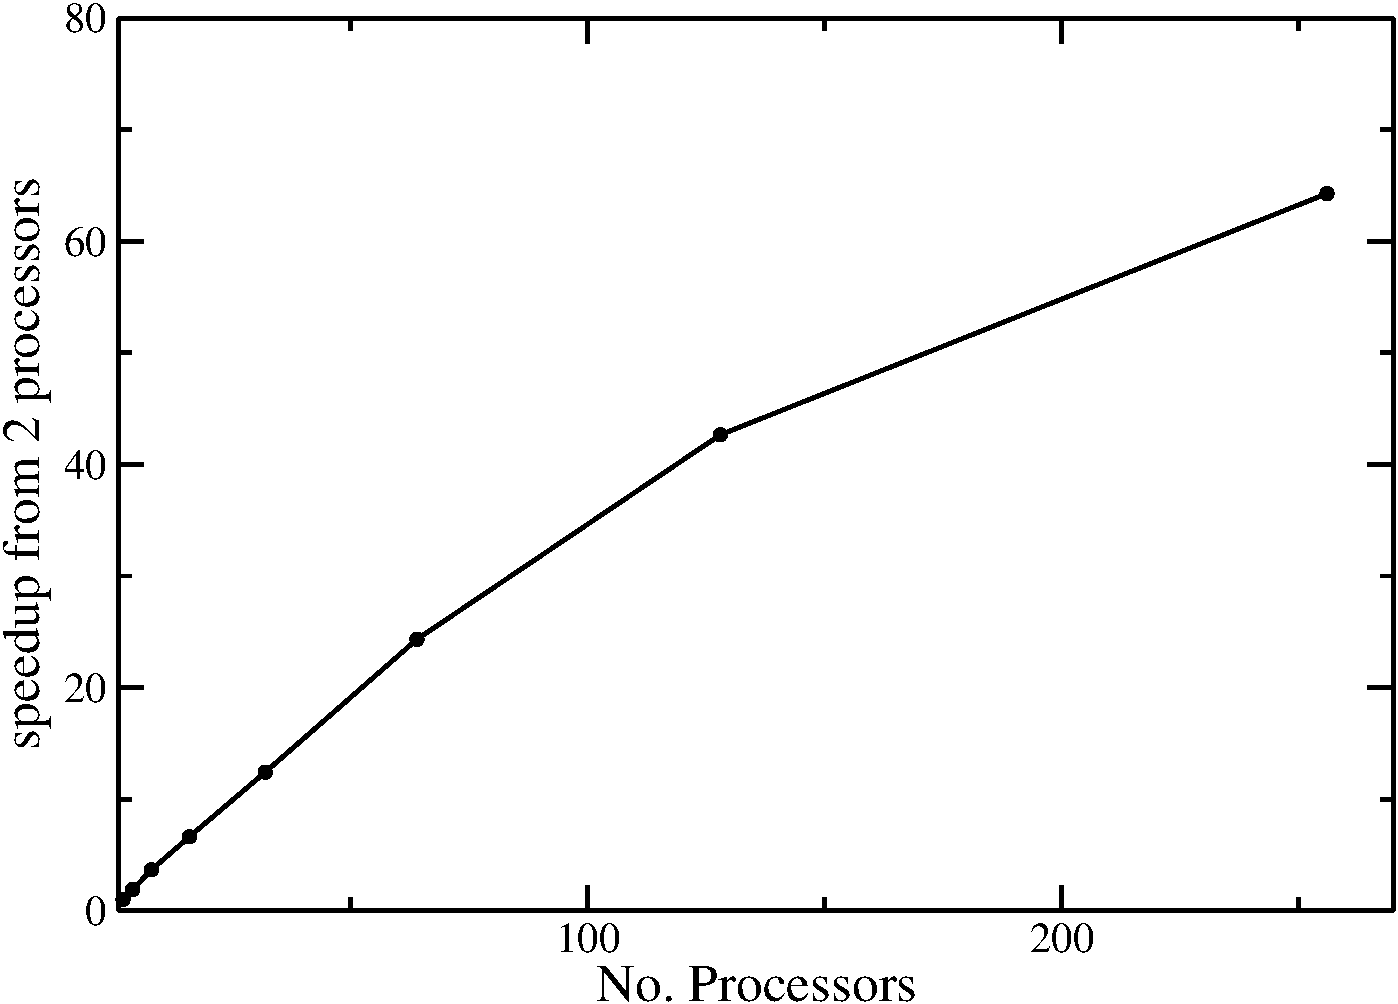
\includegraphics[scale=0.5]{efgr/benchmark}
%\caption{Benchmark of NAMD simulations for inhibitor-EGFR system}\label{fig:benchmark}
%\end{figure}
%\end{comment}
%Based on our benchmark study on Ranger (see Figure VIII of the attached `Benchmark Document'), 
%and preliminary simulations, each simulation will run optimally on 128 processors, 
%and it will consume 300 SUs/ns.
%Based on our benchmark study on Ranger (Figure \ref{fig:benchmark}), and preliminary simulations, each simulation will run optimally on 128 processors, and it will consume about 300 SUs/ns.

\item \emph{Resource requested}
Computational requirements on Ranger for intended studies of EGFR-inhibitor interaction
are listed in Table \ref{t:efgr}.

\begin{table}[h]
\centering
\begin{tabular}[b]
{|>{\scriptsize}c|>{\scriptsize}c|>{\scriptsize}
c|>{\scriptsize}c|>{\scriptsize}c|>{\scriptsize}c|>{\scriptsize}c|}
\hline
\textbf{Sim Description} & \textbf{No. Sims} &
\textbf{No. Cores} & \textbf{Disk} &
\textbf{Code} & \textbf{TG machine} & \textbf{Total SUs}\\
\hline
AEE/EGFRs (50,000 atoms) & 50$^a$ $\times$ 25$^b$ & 128 & 100GB & NAMD & Ranger & 2,000,000\\
\hline
Erlotinib/EGFRs (50,000 atoms) & 5$^c$ $\times$ 50$^a$ $\times$ 1$^b$ & 128 & 100GB & NAMD & Ranger & 400,000\\
\hline
Grand total of SUs required & & & & & & 2,400,000 \\
\hline
\end{tabular} \caption{Planned simulations and associated computational requirements. $^a$Number of replicas in one ensemble simulation; $^b$Number of simulations for each replica, each simulation lasts for 4ns; $^c$Wild-type and 4 mutant (G719S, L858R, T890M and T790M/L858R) EGFRs.}
\label{t:efgr}
\end{table}
\end{compactenum}
